\setcounter{section}{92}
\section{Определение дерева, его свойства (б/д). Определение диаметра дерева. Алгоритм поиска диаметра в дереве.}

\begin{figure}[!htb]
   \begin{minipage}{.3301\textwidth}
     \centering
     \includegraphics[height = 2 cm]{images/93-94_tree2}
     % \includegraphics[width=.7\linewidth]{93-94_example-image-a}%
     \caption{Пример дерева}
   \end{minipage}\hfill
   \begin{minipage}{.3301\textwidth}
     \centering
     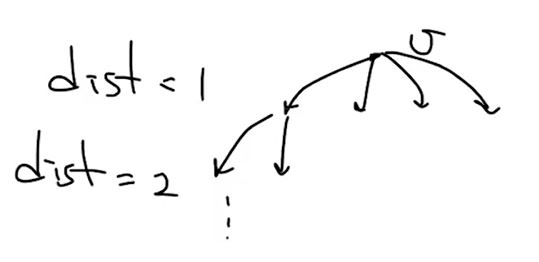
\includegraphics[height = 2 cm]{images/93-94_dfs_tree}
     \caption{DFS в дереве}
     % \includegraphics[width=.7\linewidth]{93-94_example-image-b}
     % \caption{рис.2}\label{Рис. 2}
   \end{minipage}
    \begin{minipage}{.331\textwidth}
     \centering
     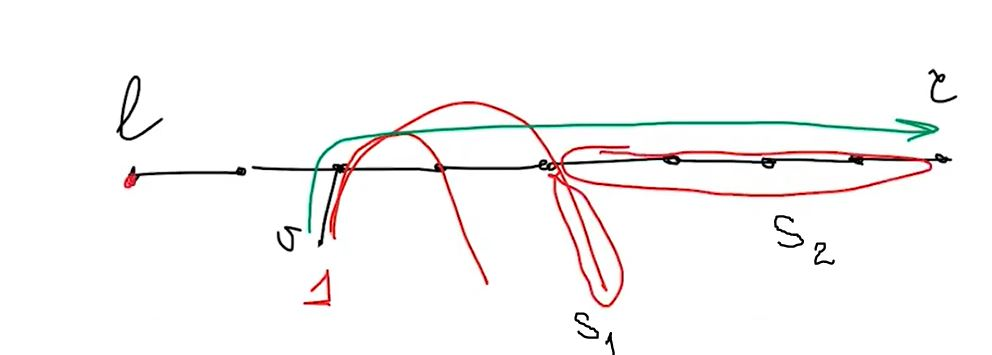
\includegraphics[height = 2 cm]{images/93-94_correct}
     \caption{Корректность поиска диаметра}
   \end{minipage}
\end{figure}

% \includegraphics[width=2cm]{93-94_tree2} \\
G - \textbf{дерево}, если G - неориентированный связный граф без циклов.\\
E(G) - рёбра графа/дерева (edges), V(G) - вершины дерева. \\
Свойства деревьев:

1. $|E(G)| = |V(G)| - 1$; количество рёбер на один меньше количества вершин дерева.

2. $\forall u, v \exists!$ простой путь из u в v. \\
\\
Пусть G - неориентированный невзвешенный граф. $dist(s, t)$ - кратчайшее расстояние между вершинами s и t. \textbf{Диаметр G} - такой путь между вершинами u и v, что $dist(u, v) = max_{s, t} dist(s, t)$. Обозначение: diam(G).

Тезис: многие задачи на графах являются очень трудными/np-трудными, а на деревьях решаются быстро. Пример 1: Поиск максимальной клики. Пример 2: Нахождение диаметра. Произвольный граф: Флойд - за $O(n^3)$. В дереве ищется за $O(n)$.

\textbf{Алгоритм поиска диаметра в дереве:}

Поиск самой далёкой вершины: "подвесим" дерево за v, дальше запускаем dfs. В силу вида дерева (см. рис. 2) мы не можем подняться на другой слой/попасть в вершину, которую мы уже посещали. Победа! - x - вершина с самого низкого уровня.

1) Пусть v - произвольная вершина. Найдём l - самую далёкую вершину от v. 

2) Теперь r - самая далёкая вершина от l. Тогда (l, r) - это диаметр.

Асимптотика: $O(n)$

Корректность: 

Посмотрим на рисунок три. Мы выбрали максимальный путь. По сути мы к каждой вершине подвесили своё дерево. Однако максимальные глубины подвешенных поддеревьев меняются в следующей последовательности: $0, 1, 2, \dots, 2, 1, 0$ (так как иначе можно найти более длинный путь). Получается, для нашей произвольной v $s_1 \leqslant s_2$. Тогда самый длинный путь из v имеет ту же длину, что путь от v до r (или до l, надо выбрать максимум). Но тогда найденная вершина находится от l на таком же расстоянии, как и r. Таким образом, мы нашли какой-то диаметр (не обязательно именно тот, который мы выбрали в начале, когда подвешивали деревья к вершинам).

\textbf{Альтернативный алгоритм}: подвесим дерево за произвольную v, среди всех деревьев-детей v выбираем самые глубокие, вершины на низших слоях этих поддеревьев будут искомыми концами диаметра.

\newpage

\setcounter{section}{93}
\section{Определение центроида в дереве. Алгоритм поиска центроида в дереве. Лемма о количестве центроидов (б/д).}

Пусть G - дерево, $v \in V(G)$. Тогда v - \textbf{центроид}, если после удаления v дерево распадается на несколько компонент, размером не более $\frac{n}{2}$

\begin{figure}[!htb]
   \begin{minipage}{.3301\textwidth}
     \centering
     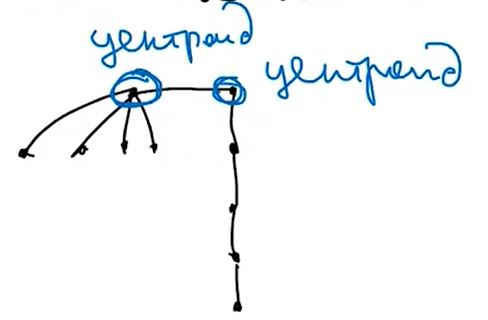
\includegraphics[height = 2 cm]{images/93-94_centroid}
     \caption{Пример центроидов}
   \end{minipage}\hfill
   \begin{minipage}{.3301\textwidth}
     \centering
     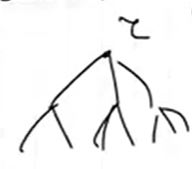
\includegraphics[height = 2 cm]{images/93-94_centroid2}
     \caption{Алгоритм поиска центроида: шаг 1}
   \end{minipage}
    \begin{minipage}{.331\textwidth}
     \centering
     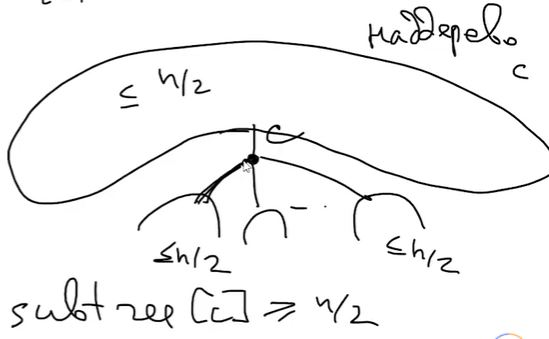
\includegraphics[height = 2 cm]{images/93-94_centroid3}
     \caption{Наддерево: шаг 2}
   \end{minipage}
\end{figure}

\textbf{Утверждение 1}. В любом дереве есть центроид.

\textbf{Утверждение 2 (б/д)}. В любом дереве либо один центроид, либо центроидов два и они соедины ребром (см. рис. 4)

\textbf{Алгоритм поиска центроида} за $O(n)$.

1. Пусть r - произвольный корень; subtree[v] = размер поддерева вершины v, включая v - это обычная динамика, dfs; subtree[r] = n. 

1.5. Цель: найти такую вершину s, размеры всех поддеревьев детей которой не больше n/2, но subtree[s] $\geqslant \frac{n}{2}$. (Наддерево также станет одним из деревьев, образованных после удаления вершины; поддерево + наддерево = всё дерево)

P.S. Дабы избавиться от бед с округлениями, лучше сравнивать не так, как записано выше, а 2subtree[s] $\geqslant n$.

2. Спускаемся от корня вниз к ребёнку с размером поддерева subtree$\cdot 2 \geqslant n$, пока можем. Как только такого ребёнка нет - вершина, где мы закончились, - центроид.